%!TEX root = /Users/zolkko/Projects/zolkko-alarm/doc/main.tex
\section*{Приложения}
\addcontentsline{toc}{section}{Приложения}
\newpage{}

% \ESKDthisStyle{formII}
\ESKDappendix{Обязательное}{Структурная схема универсальной системы терморегулирования
на базе микроконтроллера AVR семейства XMega}
\begin{figure}[h]
	\center{\includegraphics[bb=0 0 1500 2600, clip, scale=0.2]{struct_scheme.png}}
\end{figure}
\newpage{}

\ESKDappendix{Обязательное}{Принципиальная электрическая схема управляющего устройства}
\begin{figure}[h]
	\center{\includegraphics[bb=0 0 950 820, clip, scale=0.5]{scheme.png}}
\end{figure}
\newpage{}

\ESKDappendix{Обязательное}{Топологическая схема управляющего устройства}
\begin{figure}[h]
 	\center{\includegraphics[bb=0 0 450 300, clip, scale=0.9]{pcb_top_mono.png}}
	\center{\includegraphics[bb=0 0 450 300, clip, scale=0.9]{pcb_bottom_mono.png}}
\end{figure}
\newpage{}

\ESKDappendix{Обязательное}{Диаграмма классов микропрограммы микроконтроллера}
\begin{figure}[h]
	\center{\includegraphics[bb=0 0 70 70, clip, scale=7.0]{class_diagram.png}}
\end{figure}
\newpage{}

\ESKDappendix{Обязательное}{Блок-схема алгоритма терморегулирования}
\begin{figure}[h]
	\center{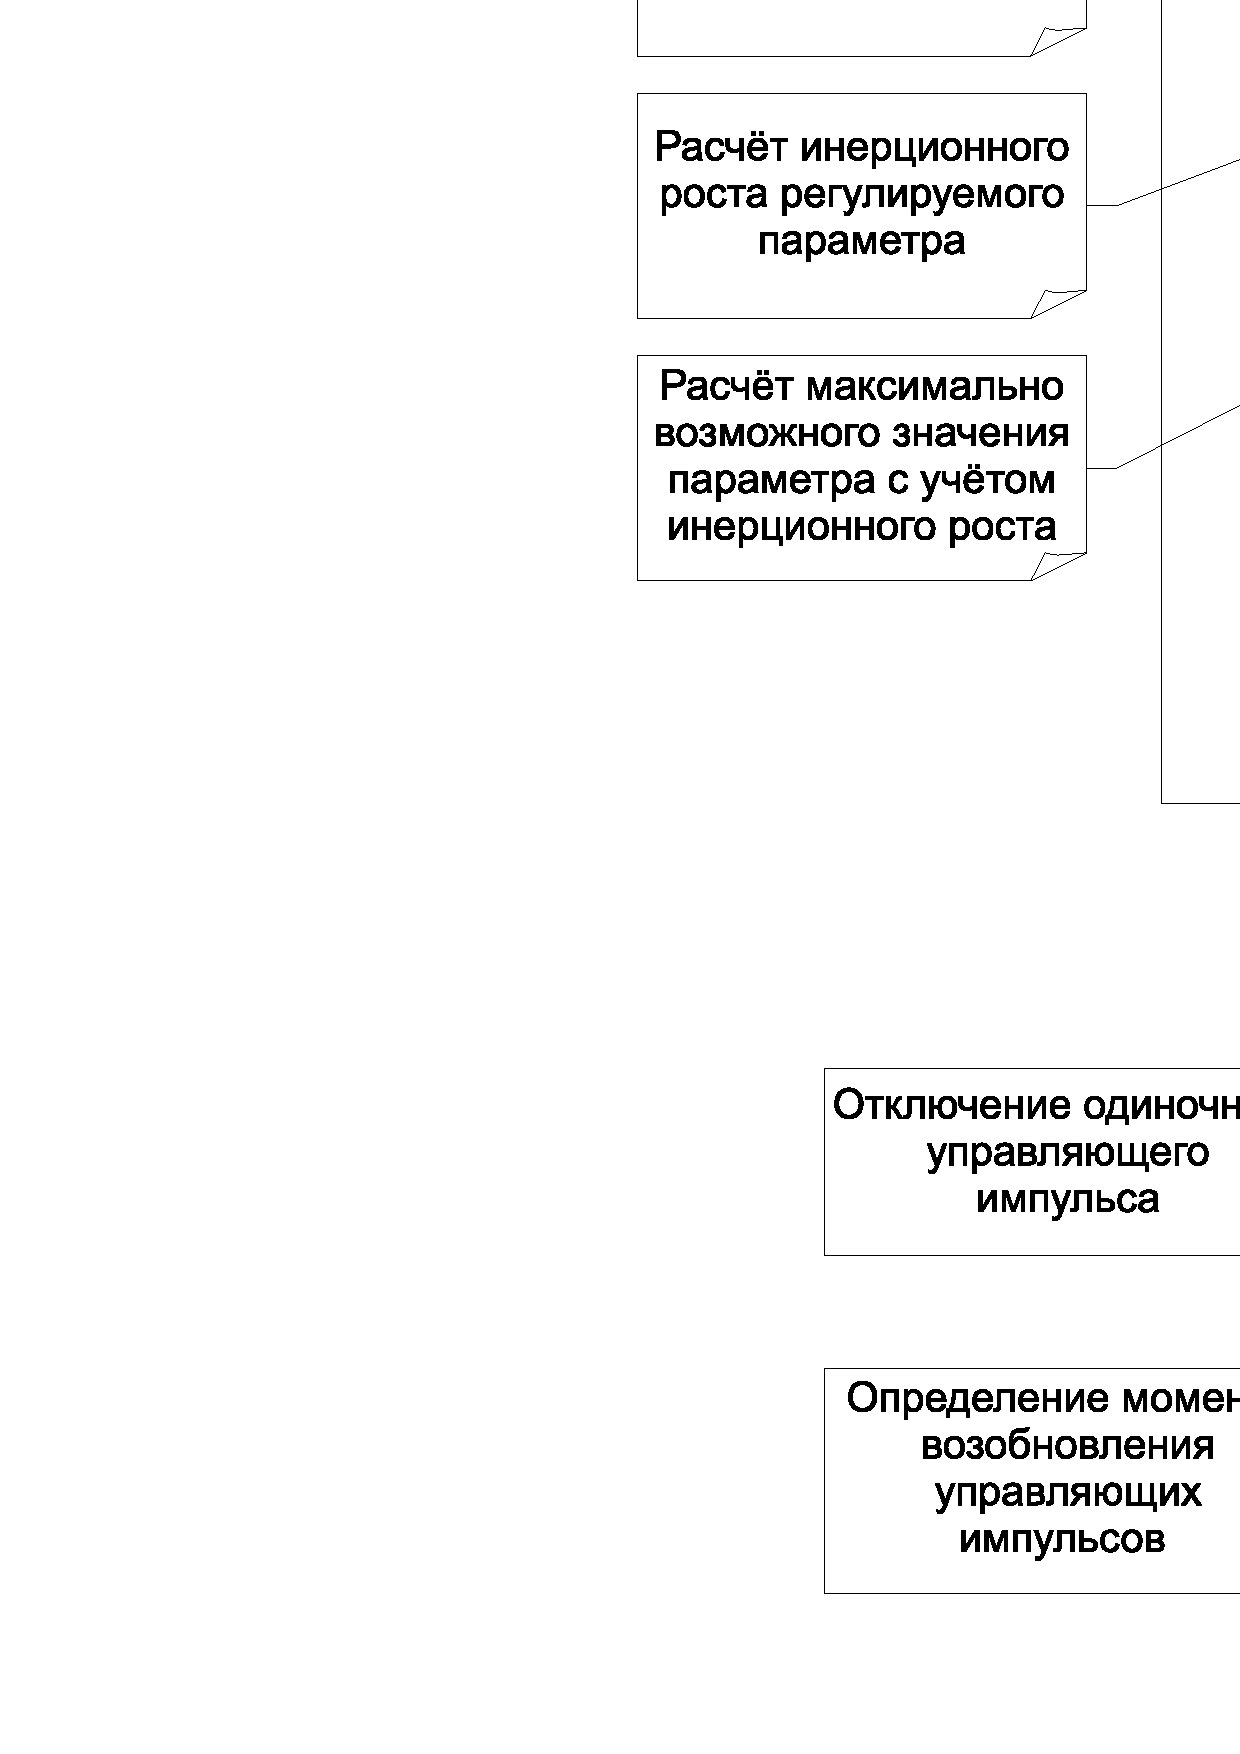
\includegraphics[bb=0 0 1500 2200, clip, scale=0.25]{algorithm.png}}
\end{figure}
\newpage{}
